% ============================================================
% PhD PROPOSAL DEFENSE PRESENTATION — NSUK CCS
% Isichei Nnamdi Augustus | PHD25DTS0002
% ML-Enhanced Portfolio Optimisation for the NGX
% ============================================================
\documentclass[aspectratio=169,11pt]{beamer}
\PassOptionsToPackage{dvipsnames,svgnames,table}{xcolor}
\usepackage[utf8]{inputenc}
\usepackage[T1]{fontenc}
\usepackage{lmodern}
\usepackage{amsmath,amssymb,amsfonts}
\usepackage{graphicx}
\usepackage{booktabs}
\usepackage{natbib}
\usepackage{tikz}
\usepackage{pgfplots}
\pgfplotsset{compat=1.18}
\usetikzlibrary{shapes.geometric,arrows.meta,positioning,
	fit,backgrounds,calc,decorations.pathreplacing}
\usepackage{colortbl}
\usepackage{multirow}
\usepackage{bm}

% ── COLOURS ────────────────────────────────────────────────
\definecolor{Navy}{HTML}{003366}
\definecolor{Gold}{HTML}{C49A00}
\definecolor{Green}{HTML}{006633}
\definecolor{Red}{HTML}{CC2200}
\definecolor{LightNavy}{HTML}{E8EEF5}
\definecolor{LightGold}{HTML}{FDF3D6}
\definecolor{LightGreen}{HTML}{E6F5ED}
\definecolor{LightRed}{HTML}{FDECEA}
\definecolor{SlateGray}{HTML}{607080}

% ── BEAMER THEME ───────────────────────────────────────────
\usetheme{Madrid}
\usecolortheme[named=Navy]{structure}
\setbeamercolor{palette primary}{bg=Navy,fg=white}
\setbeamercolor{palette secondary}{bg=Navy!85,fg=white}
\setbeamercolor{palette tertiary}{bg=Navy!70,fg=white}
\setbeamercolor{frametitle}{bg=Navy,fg=white}
\setbeamercolor{block title}{bg=Navy,fg=white}
\setbeamercolor{block body}{bg=LightNavy,fg=black}
\setbeamercolor{block title alerted}{bg=Red,fg=white}
\setbeamercolor{block body alerted}{bg=LightRed,fg=black}
\setbeamercolor{block title example}{bg=Green,fg=white}
\setbeamercolor{block body example}{bg=LightGreen,fg=black}
\setbeamercolor{itemize item}{fg=Gold}
\setbeamercolor{itemize subitem}{fg=Navy!70}
\setbeamerfont{frametitle}{size=\large,series=\bfseries}
\setbeamertemplate{navigation symbols}{}
\setbeamertemplate{itemize item}{\textbullet}
\setbeamertemplate{itemize subitem}{--}

% Gold underline on frametitle
\addtobeamertemplate{frametitle}{}{%
	\begin{tikzpicture}[remember picture,overlay]
		\draw[Gold,line width=2pt]
		(current page.north west) ++(0,-1.05cm) -- ++(16cm,0);
\end{tikzpicture}}

% Footer
\setbeamertemplate{footline}{
	\leavevmode\hbox{%
		\begin{beamercolorbox}[wd=.5\paperwidth,ht=2.25ex,dp=1ex,
			left,leftskip=1em]{palette primary}
			\tiny Isichei, N.A. | PHD24DST0004 | CCS-NSUK
		\end{beamercolorbox}%
		\begin{beamercolorbox}[wd=.3\paperwidth,ht=2.25ex,dp=1ex,
			center]{palette secondary}
			\tiny ML Portfolio Optimisation -- NGX
		\end{beamercolorbox}%
		\begin{beamercolorbox}[wd=.2\paperwidth,ht=2.25ex,dp=1ex,
			right,rightskip=1em]{palette primary}
			\tiny \insertframenumber{}/\inserttotalframenumber
\end{beamercolorbox}}}

% ── TIKZ STYLES (global — no #1 parameter) ─────────────────
\tikzset{
	arr/.style={-Stealth,thick,Navy},
	garr/.style={-Stealth,thick,Gold},
	navybox/.style={rectangle,draw=Navy,fill=LightNavy,
		rounded corners=3pt,inner sep=4pt,
		font=\scriptsize},
	greenbox/.style={rectangle,draw=Green,fill=LightGreen,
		rounded corners=3pt,inner sep=4pt,
		font=\scriptsize},
	redbox/.style={rectangle,draw=Red,fill=LightRed,
		rounded corners=3pt,inner sep=4pt,
		font=\scriptsize},
	goldbox/.style={rectangle,draw=Gold,fill=LightGold,
		rounded corners=3pt,inner sep=4pt,
		font=\scriptsize\bfseries},
}

% ── CUSTOM COMMANDS ────────────────────────────────────────
\newcommand{\hl}[1]{\textcolor{Gold}{\textbf{#1}}}
\newcommand{\bE}{\mathbb{E}}
\newcommand{\bR}{\mathbb{R}}

% ── META ───────────────────────────────────────────────────
\title[ML Portfolio Optimisation -- NGX]{%
	Machine Learning-Enhanced Portfolio Optimisation\\
	for Emerging Markets:\\
	A Two-Stage Approach for the Nigerian Stock Exchange}
\author[Isichei, N.A. | PHD24DST0004]{%
	\textbf{ISICHEI, Nnamdi Augustus} \\ {\small PHD24DST0004}}
\institute[CCS-NSUK]{%
	Centre for Cyberspace Studies\\
	Nasarawa State University, Keffi}
\date{PhD Proposal Defense, 2026}

% ===========================================================
\begin{document}
	% ===========================================================
	
	% ── SLIDE 1: TITLE ─────────────────────────────────────────
	{
		\setbeamertemplate{footline}{}
		\begin{frame}[plain]
			\begin{tikzpicture}[remember picture,overlay]
				\fill[Navy] (current page.south west) rectangle (current page.north east);
				\fill[Gold] (current page.north west) rectangle ++(16cm,-0.2cm);
				\fill[Navy!55] (current page.south west) rectangle ++(16cm,1.3cm);
			\end{tikzpicture}
			\vspace{0.15cm}
			\begin{center}
				\includegraphics[height=1.4cm]{nsuk_logo.jpg}
				\hspace{2cm}
				\includegraphics[height=1.4cm]{ccs_nsuk.jpg}\\[5pt]
				{\color{white}\rule{12cm}{0.4pt}}\\[8pt]
				{\color{Gold}\large\bfseries
					Machine Learning-Enhanced Portfolio Optimisation\\
					for Emerging Markets}\\[5pt]
				{\color{white}\normalsize
					A Two-Stage Approach for the Nigerian Stock Exchange}\\[10pt]
				{\color{white}\rule{8cm}{0.3pt}}\\[6pt]
				{\color{white}\small\bfseries ISICHEI, Nnamdi Augustus}\\
				{\color{white!75}\small PHD24DST0004}\\[4pt]
				{\color{white!65}\footnotesize
					Centre for Cyberspace Studies, Nasarawa State University, Keffi}\\[4pt]
				{\color{Gold!80}\footnotesize PhD Proposal Defense $\cdot$ 2026}
			\end{center}
		\end{frame}
	}
	
	% ── SLIDE 2: OUTLINE ───────────────────────────────────────
	\begin{frame}{Presentation Outline}
		\begin{columns}
			\column{0.48\textwidth}
			\tableofcontents[sections={1-3}]
			\column{0.48\textwidth}
			\tableofcontents[sections={4-7}]
		\end{columns}
	\end{frame}
	
	% ===========================================================
	\section{Introduction \& Problem}
	% ===========================================================
	
	% ── SLIDE 3: NGX CONTEXT ───────────────────────────────────
	\begin{frame}{The Nigerian Stock Exchange (NGX) Context}
		\begin{columns}[T]
			\column{0.50\textwidth}
			\begin{block}{Market Profile}
				\begin{itemize}\setlength\itemsep{3pt}
					\item \textbf{$\approx$150} listed equities; top 30 account
					for $>$80\% of capitalisation
					\item Thin trading volumes; lowest liquidity among
					major African exchanges
					\item Returns: \textbf{non-normal} (fat tails,
					negative skew)
					\item Strong \textbf{oil-price sensitivity} --
					petroleum drives $\approx$65\% of fiscal receipts
					\item \textbf{Naira devaluation cycles} compound
					investor risk \citep{omorokunwa2023}
				\end{itemize}
			\end{block}
			\column{0.46\textwidth}
			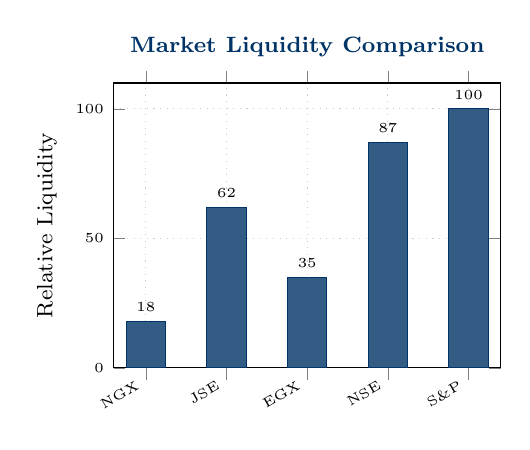
\begin{tikzpicture}
				\begin{axis}[
					width=6.5cm,height=5.2cm,
					ybar,bar width=0.5cm,
					symbolic x coords={NGX,JSE,EGX,NSE,S\&P},
					xtick=data,
					x tick label style={rotate=30,anchor=east,font=\tiny},
					ymin=0,ymax=110,
					ylabel={\footnotesize Relative Liquidity},
					ylabel style={font=\footnotesize},
					title={\footnotesize Market Liquidity Comparison},
					title style={font=\footnotesize\bfseries,color=Navy},
					grid=major,grid style={dotted,gray!40},
					nodes near coords,
					nodes near coords style={font=\tiny},
					tick label style={font=\tiny},
					]
					\addplot[fill=Navy!80,draw=Navy] coordinates
					{(NGX,18)(JSE,62)(EGX,35)(NSE,87)(S\&P,100)};
				\end{axis}
			\end{tikzpicture}\\
			{\tiny Source: \citet{omorokunwa2023}; NGX Group (2024)}
		\end{columns}
	\end{frame}
	
	% ── SLIDE 4: PROBLEM STATEMENT ─────────────────────────────
	\begin{frame}{Problem Statement}
		\vspace{-14pt}
		\begin{alertblock}{Core Research Problem}
			Classical portfolio optimisation methods consistently underperform on the NGX due to structural illiquidity, non-normal returns, and data sparsity.
			Existing ML frameworks are validated exclusively on developed or large
			Asian markets and transfer poorly to African frontier markets.
		\end{alertblock}
		\vspace{-10pt}
		\begin{columns}[T]
			\column{0.48\textwidth}
			\begin{block}{What Fails on the NGX}
				\begin{itemize}\setlength\itemsep{3pt}
					\item MVO amplifies estimation error with limited data
					\citep{markowitz2024}
					\item Static models cannot adapt to oil-shock and
					devaluation regimes
					\item No pre-selection wastes allocation on illiquid
					equities
					\item Sentiment signals from Nigerian media
					untested in literature
				\end{itemize}
			\end{block}
			\column{0.48\textwidth}
			\begin{exampleblock}{What This Study Provides}
				\begin{itemize}\setlength\itemsep{3pt}
					\item A validated \textbf{two-stage GNN-RL framework}
					for the NGX
					\item \textbf{GNN pre-selection} exploiting
					inter-stock correlation graphs
					\item \textbf{Adaptive RL allocation} with embedded
					transaction costs and liquidity constraints
					\item \textbf{Sentiment analysis} from Nigerian
					financial media (conditional)
				\end{itemize}
			\end{exampleblock}
		\end{columns}
	\end{frame}
	
	% ===========================================================
	\section{Research Design}
	% ===========================================================
	
	% ── SLIDE 5: RESEARCH QUESTIONS ────────────────────────────
	\begin{frame}{Research Questions \& Objectives}
		\vspace{0.1cm}
		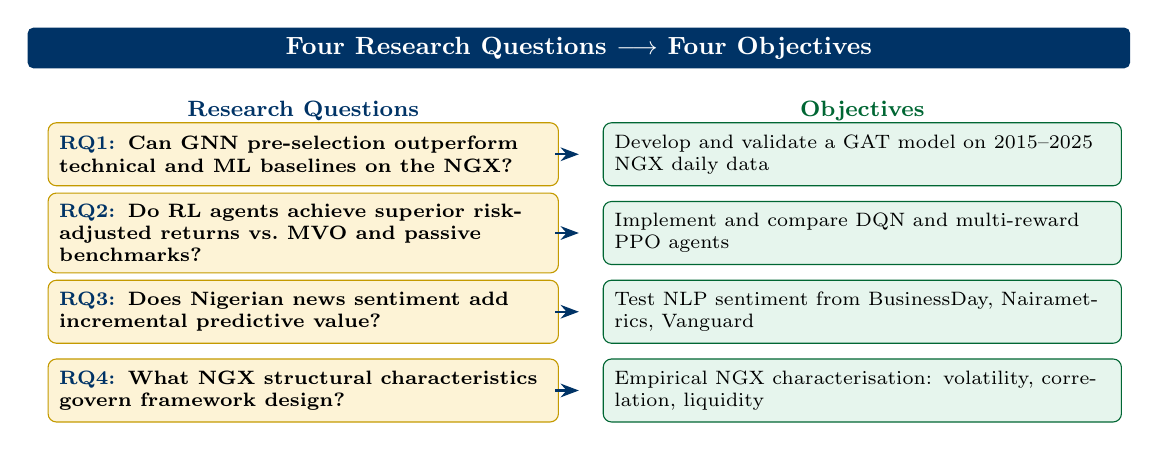
\begin{tikzpicture}
			\node[rectangle,fill=Navy,text=white,minimum width=14cm,
			minimum height=0.5cm,font=\small\bfseries,rounded corners=2pt]
			at (7,5.3) {Four Research Questions $\longrightarrow$ Four Objectives};
			
			% RQ1
			\node[goldbox,text width=6.2cm,minimum height=0.8cm,align=left]
			at (3.5,3.95)
			{\textcolor{Navy}{\bfseries RQ1:} Can GNN pre-selection outperform technical
				and ML baselines on the NGX?};
			\node[greenbox,text width=6.3cm,minimum height=0.8cm,align=left]
			at (10.6,3.95)
			{Develop and validate a GAT model on 2015--2025 NGX daily data};
			\draw[arr] (6.7,3.95) -- (7.0,3.95);
			
			% RQ2
			\node[goldbox,text width=6.2cm,minimum height=0.8cm,align=left]
			at (3.5,2.95)
			{\textcolor{Navy}{\bfseries RQ2:} Do RL agents achieve superior risk-adjusted
				returns vs.\ MVO and passive benchmarks?};
			\node[greenbox,text width=6.3cm,minimum height=0.8cm,align=left]
			at (10.6,2.95)
			{Implement and compare DQN and multi-reward PPO agents};
			\draw[arr] (6.7,2.95) -- (7.0,2.95);
			
			% RQ3
			\node[goldbox,text width=6.2cm,minimum height=0.8cm,align=left]
			at (3.5,1.95)
			{\textcolor{Navy}{\bfseries RQ3:} Does Nigerian news sentiment add
				incremental predictive value?};
			\node[greenbox,text width=6.3cm,minimum height=0.8cm,align=left]
			at (10.6,1.95)
			{Test NLP sentiment from BusinessDay, Nairametrics, Vanguard};
			\draw[arr] (6.7,1.95) -- (7.0,1.95);
			
			% RQ4
			\node[goldbox,text width=6.2cm,minimum height=0.8cm,align=left]
			at (3.5,0.95)
			{\textcolor{Navy}{\bfseries RQ4:} What NGX structural characteristics
				govern framework design?};
			\node[greenbox,text width=6.3cm,minimum height=0.8cm,align=left]
			at (10.6,0.95)
			{Empirical NGX characterisation: volatility, correlation, liquidity};
			\draw[arr] (6.7,0.95) -- (7.0,0.95);
			
			\node[font=\footnotesize\bfseries,Navy] at (3.5,4.5) {Research Questions};
			\node[font=\footnotesize\bfseries,Green] at (10.6,4.5) {Objectives};
		\end{tikzpicture}
	\end{frame}
	
	% ===========================================================
	\section{Literature Review}
	% ===========================================================
	
	% ── SLIDE 6: LITERATURE REVIEW ─────────────────────────────
	\begin{frame}{Literature Review -- Funnel Approach (16 Studies)}
		\vspace{-12pt}
		\begin{columns}
			\column{0.35\textwidth}
			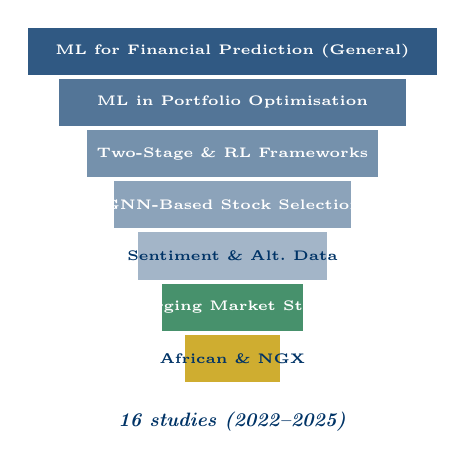
\begin{tikzpicture}
				% Layer 1 - broadest
				\fill[Navy!90,opacity=0.9] (-2.6,4.9) rectangle (2.6,5.5);
				\node[white,font=\tiny\bfseries,align=center] at (0,5.2)
				{ML for Financial Prediction (General)};
				% Layer 2
				\fill[Navy!75,opacity=0.9] (-2.2,4.25) rectangle (2.2,4.85);
				\node[white,font=\tiny\bfseries,align=center] at (0,4.55)
				{ML in Portfolio Optimisation};
				% Layer 3
				\fill[Navy!60,opacity=0.9] (-1.85,3.6) rectangle (1.85,4.2);
				\node[white,font=\tiny\bfseries,align=center] at (0,3.9)
				{Two-Stage \& RL Frameworks};
				% Layer 4
				\fill[Navy!50,opacity=0.9] (-1.5,2.95) rectangle (1.5,3.55);
				\node[white,font=\tiny\bfseries,align=center] at (0,3.25)
				{GNN-Based Stock Selection};
				% Layer 5
				\fill[Navy!40,opacity=0.9] (-1.2,2.3) rectangle (1.2,2.9);
				\node[Navy,font=\tiny\bfseries,align=center] at (0,2.6)
				{Sentiment \& Alt.\ Data};
				% Layer 6
				\fill[Green!80,opacity=0.9] (-0.9,1.65) rectangle (0.9,2.25);
				\node[white,font=\tiny\bfseries,align=center] at (0,1.95)
				{Emerging Market Studies};
				% Layer 7 - most specific
				\fill[Gold!90,opacity=0.9] (-0.6,1.0) rectangle (0.6,1.6);
				\node[Navy,font=\tiny\bfseries,align=center] at (0,1.3)
				{African \& NGX};
				\node[font=\scriptsize\bfseries,Navy] at (0,0.5)
				{\textit{16 studies (2022--2025)}};
			\end{tikzpicture}
			
			\column{0.62\textwidth}
			\begin{block}{Key Findings by Strand}
				\begin{itemize}\setlength\itemsep{4pt}
					\item GNNs consistently outperform non-relational
					baselines \citep{patel2024}
					\item Two-stage frameworks dominate single-stage
					optimisation \citep{huang2024}
					\item Multi-reward RL: 124.83\% return on Indian NSE
					\citep{orra2025}
					\item BiLSTM-GAT superior for stock prediction
					\citep{lu2025}
					\item NGX volatility negatively affects returns;
					liquidity is positive predictor
					\citep{omorokunwa2023}
					\item Investor sentiment significantly related to
					NGX returns \citep{john2022}
				\end{itemize}
			\end{block}
		\end{columns}
	\end{frame}
	
	% ── SLIDE 7: RESEARCH GAPS ─────────────────────────────────
	\begin{frame}{Identified Research Gaps}
		\begin{center}
		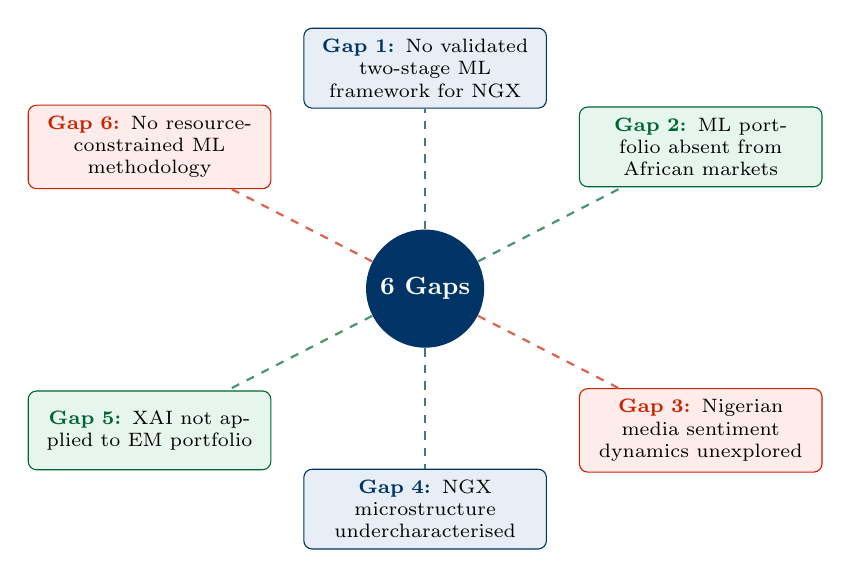
\begin{tikzpicture}
			\node[circle,fill=Navy,text=white,minimum size=1.5cm,
			font=\small\bfseries,align=center] (C) at (7,3.0)
			{6 Gaps};
			% Gap 1 - top
			\node[navybox,text width=2.8cm,minimum height=1.0cm,align=center]
			(G1) at (7,5.8)
			{\textcolor{Navy}{\bfseries Gap 1:} No validated two-stage ML framework for NGX};
			\draw[Navy!70,thick,dashed] (C) -- (G1);
			% Gap 2 - top right
			\node[greenbox,text width=2.8cm,minimum height=1.0cm,align=center]
			(G2) at (10.5,4.8)
			{\textcolor{Green}{\bfseries Gap 2:} ML portfolio absent from African markets};
			\draw[Green!70,thick,dashed] (C) -- (G2);
			% Gap 3 - bottom right
			\node[redbox,text width=2.8cm,minimum height=1.0cm,align=center]
			(G3) at (10.5,1.2)
			{\textcolor{Red}{\bfseries Gap 3:} Nigerian media sentiment dynamics unexplored};
			\draw[Red!70,thick,dashed] (C) -- (G3);
			% Gap 4 - bottom
			\node[navybox,text width=2.8cm,minimum height=1.0cm,align=center]
			(G4) at (7,0.2)
			{\textcolor{Navy}{\bfseries Gap 4:} NGX microstructure undercharacterised};
			\draw[Navy!70,thick,dashed] (C) -- (G4);
			% Gap 5 - bottom left
			\node[greenbox,text width=2.8cm,minimum height=1.0cm,align=center]
			(G5) at (3.5,1.2)
			{\textcolor{Green}{\bfseries Gap 5:} XAI not applied to EM portfolio};
			\draw[Green!70,thick,dashed] (C) -- (G5);
			% Gap 6 - top left
			\node[redbox,text width=2.8cm,minimum height=1.0cm,align=center]
			(G6) at (3.5,4.8)
			{\textcolor{Red}{\bfseries Gap 6:} No resource-constrained ML methodology};
			\draw[Red!70,thick,dashed] (C) -- (G6);
		\end{tikzpicture}
	\end{center}
	\end{frame}
	
	% ===========================================================
	\section{Theoretical Framework}
	% ===========================================================
	
	% ── SLIDE 8: THEORETICAL FRAMEWORK ─────────────────────────
	\begin{frame}{Theoretical Framework -- Six Pillars}
		\begin{center}
		\vspace{0.1cm}
		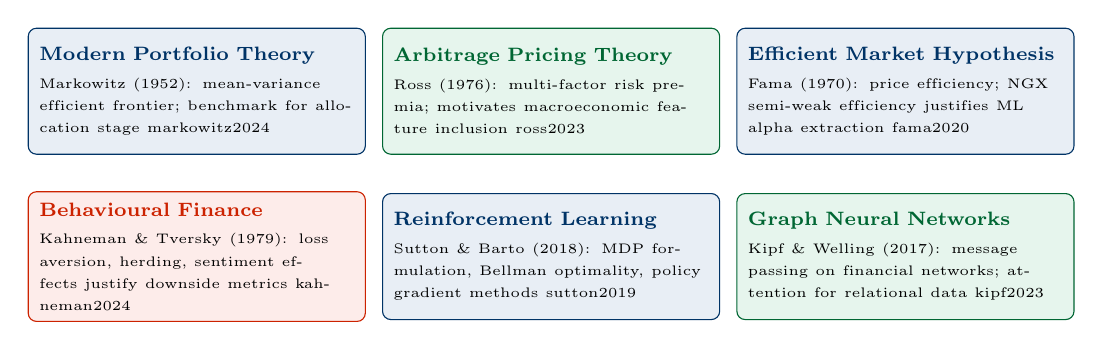
\begin{tikzpicture}
			% Row 1 (top)
			\node[navybox,text width=4.0cm,minimum height=1.6cm,align=left]
			at (1.7,3.3)
			{\textcolor{Navy}{\bfseries Modern Portfolio Theory}\\[2pt]
				\tiny Markowitz (1952): mean-variance efficient frontier; benchmark for allocation stage \citep{markowitz2024}};
			\node[greenbox,text width=4.0cm,minimum height=1.6cm,align=left]
			at (6.2,3.3)
			{\textcolor{Green}{\bfseries Arbitrage Pricing Theory}\\[2pt]
				\tiny Ross (1976): multi-factor risk premia; motivates macroeconomic feature inclusion \citep{ross2023}};
			\node[navybox,text width=4.0cm,minimum height=1.6cm,align=left]
			at (10.7,3.3)
			{\textcolor{Navy}{\bfseries Efficient Market Hypothesis}\\[2pt]
				\tiny Fama (1970): price efficiency; NGX semi-weak efficiency justifies ML alpha extraction \citep{fama2020}};
			% Row 2 (bottom)
			\node[redbox,text width=4.0cm,minimum height=1.6cm,align=left]
			at (1.7,1.2)
			{\textcolor{Red}{\bfseries Behavioural Finance}\\[2pt]
				\tiny Kahneman \& Tversky (1979): loss aversion, herding, sentiment effects justify downside metrics \citep{kahneman2024}};
			\node[navybox,text width=4.0cm,minimum height=1.6cm,align=left]
			at (6.2,1.2)
			{\textcolor{Navy}{\bfseries Reinforcement Learning}\\[2pt]
				\tiny Sutton \& Barto (2018): MDP formulation, Bellman optimality, policy gradient methods \citep{sutton2019}};
			\node[greenbox,text width=4.0cm,minimum height=1.6cm,align=left]
			at (10.7,1.2)
			{\textcolor{Green}{\bfseries Graph Neural Networks}\\[2pt]
				\tiny Kipf \& Welling (2017): message passing on financial networks; attention for relational data \citep{kipf2023}};
		\end{tikzpicture}
	\end{center}
	\end{frame}
	
	% ===========================================================
	\section{Proposed Framework}
	% ===========================================================
	
	% ── SLIDE 9: TWO-STAGE ARCHITECTURE (IMPROVED) ─────────────
	\begin{frame}{Proposed Two-Stage GNN-RL Framework}
		\begin{center}
			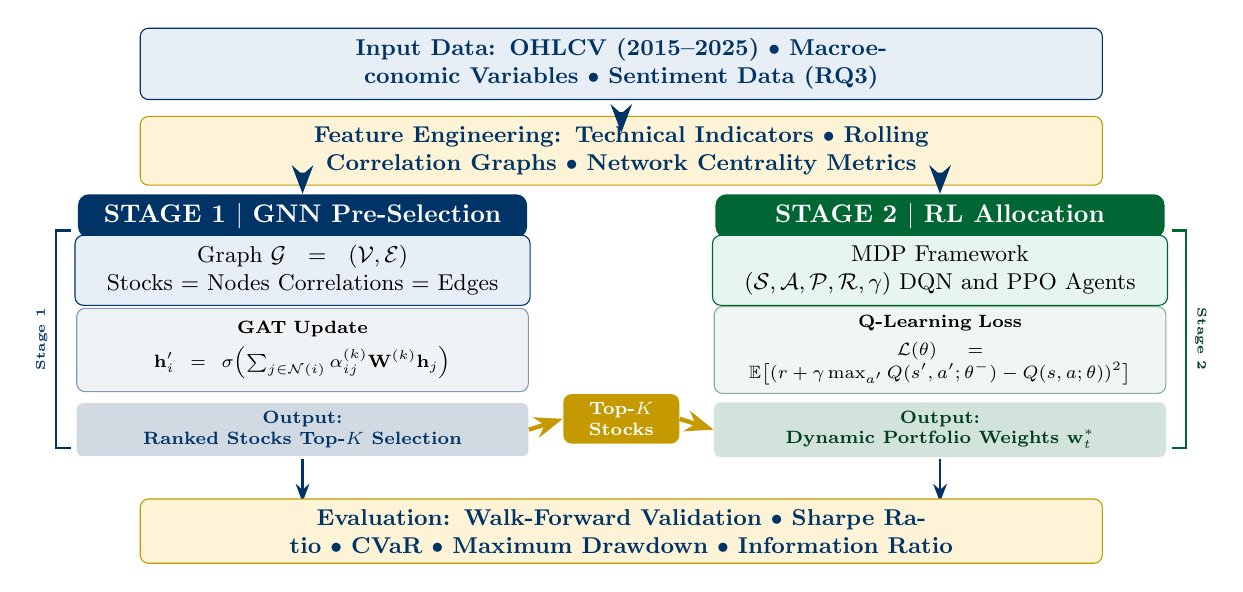
\begin{tikzpicture}[scale=0.92,transform shape]
				
				%% ── DATA INPUT LAYER ──────────────────────────────────────
				
				\node[navybox,
				text width=13cm,
				minimum height=0.72cm,
				font=\small\bfseries,
				text=Navy,
				align=center]
				(data) at (7,6.0)
				{\textbf{Input Data:}
					OHLCV (2015--2025) $\bullet$
					Macroeconomic Variables $\bullet$
					Sentiment Data (RQ3)};
				
				\node[goldbox,
				text width=13cm,
				minimum height=0.60cm,
				font=\small\bfseries,
				text=Navy,
				align=center]
				(feat) at (7,4.8)
				{Feature Engineering:
					Technical Indicators $\bullet$
					Rolling Correlation Graphs $\bullet$
					Network Centrality Metrics};
				
				\draw[arr,ultra thick]
				(7,5.34) -- (7,5.05);
				
				%% ── STAGE 1 PANEL ────────────────────────────────────────
				
				\node[
				rectangle,
				fill=Navy,
				text=white,
				rounded corners=4pt,
				minimum width=6.2cm,
				minimum height=0.60cm,
				font=\normalsize\bfseries]
				(s1h) at (2.6,3.9)
				{STAGE 1 $|$ GNN Pre-Selection};
				
				\draw[arr,ultra thick]
				(2.6,4.50) -- (s1h.north);
				
				\node[navybox,
				text width=6.0cm,
				minimum height=0.8cm,
				font=\small,
				align=center]
				(s1c) at (2.6,3.15)
				{Graph $\mathcal{G}=(\mathcal{V},\mathcal{E})$\\
					Stocks = Nodes
					Correlations = Edges};
				
				\node[
				rectangle,
				draw=Navy!50,
				fill=Navy!6,
				rounded corners=3pt,
				text width=6.0cm,
				minimum height=1.15cm,
				font=\scriptsize,
				align=center]
				(s1eq) at (2.6,2.05)
				{\textbf{GAT Update}\\[3pt]
					$
					\mathbf h_i'=
					\sigma\!\left(
					\sum_{j\in\mathcal N(i)}
					\alpha_{ij}^{(k)}
					\mathbf W^{(k)}
					\mathbf h_j
					\right)
					$
				};
				
				\node[
				rectangle,
				fill=Navy!18,
				rounded corners=2pt,
				text width=6.0cm,
				minimum height=0.65cm,
				font=\scriptsize\bfseries,
				text=Navy,
				align=center]
				(s1o) at (2.6,0.95)
				{Output:\\
					Ranked Stocks
					Top-$K$ Selection};
				
				%% Stage 1 Bracket
				
				\draw[Navy,thick]
				(-0.6,3.7) --
				(-0.8,3.7) --
				(-0.8,0.7) --
				(-0.6,0.7);
				
				\node[
				rotate=90,
				font=\tiny\bfseries,
				Navy]
				at (-1.0,2.2)
				{Stage 1};
				
				%% ── CONNECTOR ────────────────────────────────────────────
				
				\node[
				rectangle,
				fill=Gold,
				text=white,
				rounded corners=3pt,
				minimum width=1.6cm,
				minimum height=0.65cm,
				font=\scriptsize\bfseries,
				align=center]
				(conn) at (7,1.1)
				{Top-$K$\\Stocks};
				
				\draw[garr,ultra thick]
				(s1o.east) -- (conn.west);
				
				%% ── STAGE 2 PANEL ────────────────────────────────────────
				
				\node[
				rectangle,
				fill=Green,
				text=white,
				rounded corners=4pt,
				minimum width=6.2cm,
				minimum height=0.60cm,
				font=\normalsize\bfseries]
				(s2h) at (11.4,3.9)
				{STAGE 2 $|$ RL Allocation};
				
				\draw[arr,ultra thick]
				(11.4,4.50) -- (s2h.north);
				
				\node[greenbox,
				text width=6.0cm,
				minimum height=0.8cm,
				font=\small,
				align=center]
				(s2c) at (11.4,3.15)
				{MDP Framework\\
					$(\mathcal S,\mathcal A,\mathcal P,\mathcal R,\gamma)$
					DQN and PPO Agents};
				
				\node[
				rectangle,
				draw=Green!50,
				fill=Green!6,
				rounded corners=3pt,
				text width=6.0cm,
				minimum height=1.15cm,
				font=\scriptsize,
				align=center]
				(s2eq) at (11.4,2.05)
				{\textbf{Q-Learning Loss}\\[3pt]
					$
					\mathcal L(\theta)=
					\mathbb E\!\left[
					(r+\gamma\max_{a'}
					Q(s',a';\theta^-)
					-Q(s,a;\theta))^2
					\right]
					$
				};
				
				\node[
				rectangle,
				fill=Green!18,
				rounded corners=2pt,
				text width=6.0cm,
				minimum height=0.65cm,
				font=\scriptsize\bfseries,
				text=Green!60!black,
				align=center]
				(s2o) at (11.4,0.95)
				{Output:\\
					Dynamic Portfolio
					Weights $\mathbf w_t^*$};
				
				\draw[garr,ultra thick]
				(conn.east) -- (s2o.west);
				
				%% Stage 2 Bracket
				
				\draw[Green,thick]
				(14.6,3.7) --
				(14.8,3.7) --
				(14.8,0.7) --
				(14.6,0.7);
				
				\node[
				rotate=270,
				font=\tiny\bfseries,
				Green!60!black]
				at (15.0,2.2)
				{Stage 2};
				
				%% ── EVALUATION BAR ───────────────────────────────────────
				
				\draw[arr,thick]
				(2.6,0.55) -- (2.6,-0.05);
				
				\draw[arr,thick]
				(11.4,0.55) -- (11.4,-0.05);
				
				\node[goldbox,
				text width=13cm,
				minimum height=0.70cm,
				font=\small\bfseries,
				text=Navy,
				align=center]
				at (7,-0.45)
				{Evaluation:
					Walk-Forward Validation $\bullet$
					Sharpe Ratio $\bullet$
					CVaR $\bullet$
					Maximum Drawdown $\bullet$
					Information Ratio};
				
			\end{tikzpicture}
		\end{center}
	\end{frame}
	
	% ===========================================================
	\section{Model Specification}
	% ===========================================================
	
	% ── SLIDE 10: GAT DETAIL ───────────────────────────────────
	\begin{frame}{Stage 1 -- Graph Attention Network (GAT)}
		\vspace{-10pt}
		\begin{columns}[T]
			\column{0.50\textwidth}
			\begin{block}{Architecture \& Training}
				\begin{itemize}\setlength\itemsep{3pt}
					\item \textbf{3-layer GAT}: 8 heads (64 feat),
					8 heads (32 feat), 1 head (output)
					\item Activation: ELU; Dropout: 0.3
					\item Graph: 60-day rolling Pearson correlation;
					threshold $\theta=0.3$
					\item Loss: Pairwise Ranking Loss
					\item Optimiser: Adam ($\eta=0.001$);
					early stopping patience 20 epochs
				\end{itemize}
			\end{block}
			{\small Attention score:}
			\[e_{ij}^{(k)} = \text{LeakyReLU}\!\bigl(
			\mathbf{a}^{(k)\top}[\mathbf{W}^{(k)}\mathbf{h}_i
			\| \mathbf{W}^{(k)}\mathbf{h}_j]\bigr)\]
			
			\column{0.40\textwidth}
			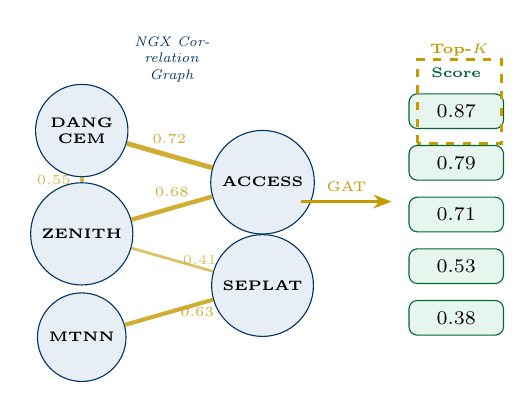
\begin{tikzpicture}[scale=0.82]
				% Stock nodes
				\node[circle,draw=Navy,fill=LightNavy,minimum size=0.9cm,
				font=\tiny\bfseries,align=center] (n1) at (0,4.2) {DANG\\CEM};
				\node[circle,draw=Navy,fill=LightNavy,minimum size=0.9cm,
				font=\tiny\bfseries] (n2) at (0,2.6) {ZENITH};
				\node[circle,draw=Navy,fill=LightNavy,minimum size=0.9cm,
				font=\tiny\bfseries] (n3) at (0,1.0) {MTNN};
				\node[circle,draw=Navy,fill=LightNavy,minimum size=0.9cm,
				font=\tiny\bfseries] (n4) at (2.8,3.4) {ACCESS};
				\node[circle,draw=Navy,fill=LightNavy,minimum size=0.9cm,
				font=\tiny\bfseries] (n5) at (2.8,1.8) {SEPLAT};
				% Weighted edges
				\draw[Gold,line width=1.8pt,opacity=0.8] (n1) -- (n4)
				node[midway,above,font=\tiny]{0.72};
				\draw[Gold,line width=1.3pt,opacity=0.7] (n1) -- (n2)
				node[midway,left,font=\tiny]{0.55};
				\draw[Gold,line width=1.6pt,opacity=0.8] (n2) -- (n4)
				node[midway,above,font=\tiny]{0.68};
				\draw[Gold,line width=1.0pt,opacity=0.6] (n2) -- (n5)
				node[midway,right,font=\tiny]{0.41};
				\draw[Gold,line width=1.5pt,opacity=0.8] (n3) -- (n5)
				node[midway,right,font=\tiny]{0.63};
				% Output scores
				\node[greenbox,minimum width=1.2cm] (o4) at (5.8,4.5)
				{0.87};
				\node[greenbox,minimum width=1.2cm] (o1) at (5.8,3.7)
				{0.79};
				\node[greenbox,minimum width=1.2cm] (o2) at (5.8,2.9)
				{0.71};
				\node[greenbox,minimum width=1.2cm] (o5) at (5.8,2.1)
				{0.53};
				\node[greenbox,minimum width=1.2cm] (o3) at (5.8,1.3)
				{0.38};
				\node[font=\tiny\bfseries,Green] at (5.8,5.1) {Score};
				\draw[garr,thick] (3.4,3.1) -- (4.8,3.1)
				node[midway,above,font=\tiny]{GAT};
				% Top-K box
				\draw[Gold,thick,dashed] (5.2,4.0) rectangle (6.5,5.3);
				\node[font=\tiny\bfseries,Gold] at (5.85,5.45) {Top-$K$};
				\node[font=\tiny,Navy,align=center,text width=1.5cm] at (1.4,5.3)
				{\textit{NGX Correlation}\\\textit{Graph}};
			\end{tikzpicture}\\
			{\tiny \citet{patel2024}; \citet{lu2025}}
			{\small Normalised weight:}
			\[\alpha_{ij}^{(k)} = \frac{\exp(e_{ij}^{(k)})}
			{\sum_{m\in\mathcal{N}(i)}\exp(e_{im}^{(k)})}\]
		\end{columns}
	\end{frame}
	
	% ── SLIDE 11: RL FRAMEWORK ─────────────────────────────────
	\begin{frame}{Stage 2 -- Reinforcement Learning Allocation}
		\vspace{-12pt}
		\begin{columns}[T]
			\column{0.52\textwidth}
			\begin{block}{MDP Formulation}
				{\small
					\begin{itemize}\setlength\itemsep{2pt}
						\item \textbf{State} $s_t$: weights $\mathbf{w}_t$, cash $c_t$,
						price and technical features
						\item \textbf{Action} $a_t\in[-1,1]^K$: weight changes
						\item \textbf{Multi-objective Reward:}
				\end{itemize}}
				\[R_t = \alpha_1 r_t + \alpha_2\frac{\bar{r}_t}{\hat{\sigma}_t}
				- \alpha_3\hat{\sigma}_t - \alpha_4\text{DD}_t
				- \alpha_5\text{Turnover}_t\]
				{\small\textbf{Constraints:} $\sum w_i=1$, $w_i\geq0$,
					$w_i\leq20\%$, $w_i\geq2\%$}
			\end{block}
			
			\begin{exampleblock}{Algorithms}
				{\small
					\begin{itemize}\setlength\itemsep{1pt}
						\item \textbf{DQN} \citep{mnih2019}: experience replay
						+ target network
						\item \textbf{Ensemble}: 3 agents (return, Sharpe, drawdown)
						\citep{orra2025}
				\end{itemize}}
			\end{exampleblock}
			
			\column{0.40\textwidth}
			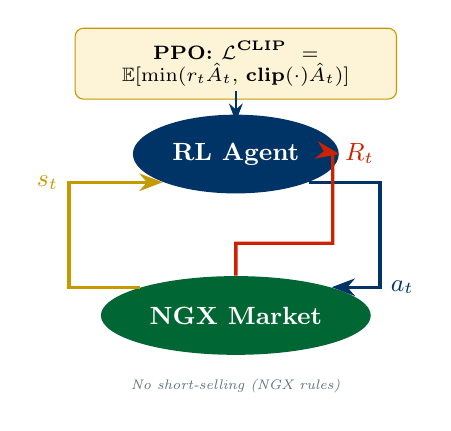
\begin{tikzpicture}[scale=0.82]
				\node[ellipse,fill=Navy,text=white,minimum width=2.4cm,
				minimum height=1.0cm,font=\small\bfseries] (A) at (3.5,4.0)
				{RL Agent};
				\node[ellipse,fill=Green,text=white,minimum width=2.4cm,
				minimum height=1.0cm,font=\small\bfseries] (E) at (3.5,1.5)
				{NGX Market};
				% State
				\draw[Gold,very thick,-Stealth]
				(E.north west) -- +(-1.1,0) |- (A.south west)
				node[midway,left,font=\small,Gold]{$s_t$};
				% Action
				\draw[Navy,very thick,-Stealth]
				(A.south east) -- +(1.1,0) |- (E.north east)
				node[midway,right,font=\small,Navy]{$a_t$};
				% Reward
				\draw[Red,very thick,-Stealth]
				(E.north) -- +(0,0.5) -- +(1.5,0.5) -- +(1.5,1.9)
				-- (A.east)
				node[near start,right,font=\small,Red]{$R_t$};
				% PPO objective
				\node[goldbox,text width=3.8cm,minimum height=0.9cm,
				align=center] at (3.5,5.4)
				{\textbf{PPO:} $\mathcal{L}^{\text{CLIP}}=
					\bE[\min(r_t\hat{A}_t,\,\text{clip}(\cdot)\hat{A}_t)]$};
				\draw[arr] (3.5,4.98) -- (3.5,4.5);
				\node[font=\tiny,SlateGray,align=center] at (3.5,0.4)
				{\textit{No short-selling (NGX rules)}};
			\end{tikzpicture}
		
			\begin{exampleblock}{Algorithms}
				{\small
					\begin{itemize}\setlength\itemsep{2pt}
						\item \textbf{PPO} \citep{schulman2019}: clipped surrogate,
						actor-critic architecture
				\end{itemize}}
			\end{exampleblock}
		\end{columns}
	\end{frame}
	
	% ===========================================================
	\section{Methodology \& Data}
	% ===========================================================
	
	% ── SLIDE 12: METHODOLOGY ──────────────────────────────────
	\begin{frame}{Research Methodology -- Six Phases}
		\begin{center}
		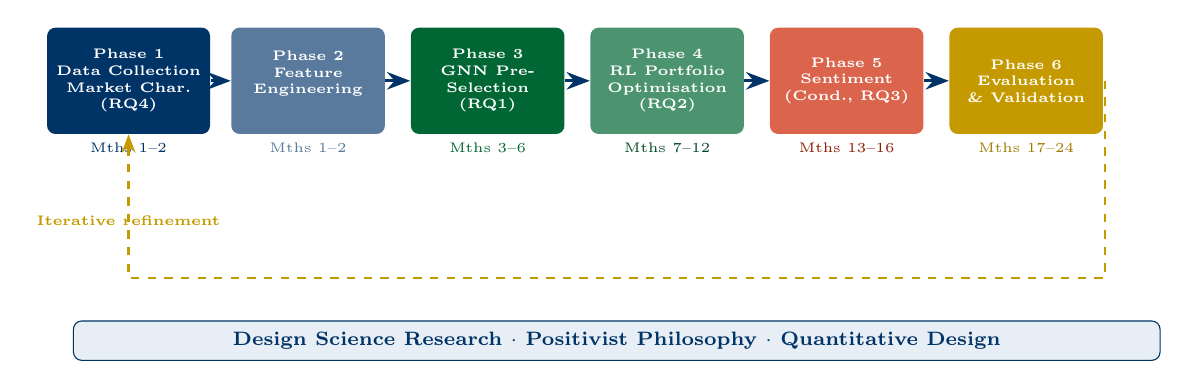
\begin{tikzpicture}
			% Phase boxes — hardcoded colours
			\node[rectangle,fill=Navy,text=white,rounded corners=3pt,
			minimum width=1.95cm,minimum height=1.35cm,
			font=\tiny\bfseries,align=center] (P1) at (0.8,3.5)
			{Phase 1\\Data Collection\\Market Char.\\(RQ4)};
			\node[rectangle,fill=Navy!65,text=white,rounded corners=3pt,
			minimum width=1.95cm,minimum height=1.35cm,
			font=\tiny\bfseries,align=center] (P2) at (3.08,3.5)
			{Phase 2\\Feature\\Engineering\\};
			\node[rectangle,fill=Green,text=white,rounded corners=3pt,
			minimum width=1.95cm,minimum height=1.35cm,
			font=\tiny\bfseries,align=center] (P3) at (5.36,3.5)
			{Phase 3\\GNN Pre-\\Selection\\(RQ1)};
			\node[rectangle,fill=Green!70,text=white,rounded corners=3pt,
			minimum width=1.95cm,minimum height=1.35cm,
			font=\tiny\bfseries,align=center] (P4) at (7.64,3.5)
			{Phase 4\\RL Portfolio\\Optimisation\\(RQ2)};
			\node[rectangle,fill=Red!70,text=white,rounded corners=3pt,
			minimum width=1.95cm,minimum height=1.35cm,
			font=\tiny\bfseries,align=center] (P5) at (9.92,3.5)
			{Phase 5\\Sentiment\\(Cond., RQ3)};
			\node[rectangle,fill=Gold,text=white,rounded corners=3pt,
			minimum width=1.95cm,minimum height=1.35cm,
			font=\tiny\bfseries,align=center] (P6) at (12.2,3.5)
			{Phase 6\\Evaluation\\\& Validation};
			
			% Arrows
			\draw[arr,very thick] (P1.east) -- (P2.west);
			\draw[arr,very thick] (P2.east) -- (P3.west);
			\draw[arr,very thick] (P3.east) -- (P4.west);
			\draw[arr,very thick] (P4.east) -- (P5.west);
			\draw[arr,very thick] (P5.east) -- (P6.west);
			
			% Period labels
			\node[font=\tiny,Navy] at (0.8,2.65) {Mths 1--2};
			\node[font=\tiny,Navy!65] at (3.08,2.65) {Mths 1--2};
			\node[font=\tiny,Green] at (5.36,2.65) {Mths 3--6};
			\node[font=\tiny,Green!70!black] at (7.64,2.65) {Mths 7--12};
			\node[font=\tiny,Red!70!black] at (9.92,2.65) {Mths 13--16};
			\node[font=\tiny,Gold!80!black] at (12.2,2.65) {Mths 17--24};
			
			% Feedback arrow
			\draw[garr,dashed,thick]
			(13.2,3.5) -- (13.2,1.0) -- (0.8,1.0) -- (0.8,2.82)
			node[midway,below,font=\tiny\bfseries,Gold]{Iterative refinement};
			
			% DSR label
			\node[navybox,minimum width=13.8cm,minimum height=0.5cm,
			font=\scriptsize\bfseries,text=Navy] at (7,0.2)
			{Design Science Research $\cdot$ Positivist Philosophy
				$\cdot$ Quantitative Design};
		\end{tikzpicture}
		\end{center}
	\end{frame}
	
	% ── SLIDE 13: DATA & EVALUATION (IMPROVED) ─────────────────
	\begin{frame}{Data Collection \& Evaluation Framework}
		\vspace{-14pt}
		%% ── TOP ROW: two info blocks side by side ──────────────────
		\begin{columns}[T]
			\column{0.42\textwidth}
			\vspace{-2pt}
			\begin{block}{Data Sources}
				{\scriptsize
					\begin{tabular}{ll}
						\toprule
						\textbf{Source} & \textbf{Variables}\\
						\midrule
						NGX Portal      & OHLCV (30--50 equities)\\
						CBN             & MPR, NGN/USD Rate\\
						NBS             & CPI, GDP Growth\\
						EIA             & Brent Crude Spot Price\\
						CBOE/FRED       & VIX, US 10-Year Yield\\
						NLP Scraper     & News Sentiment (RQ3)\\
						\bottomrule
					\end{tabular}\\[3pt]
					\textbf{Period:} Jan 2015 -- Dec 2025
					($\approx$\,2,500 trading days)}
			\end{block}
			
			\column{0.55\textwidth}
			\vspace{-2pt}
			\begin{block}{Evaluation Metrics}
				{\scriptsize
					\begin{tabular}{ll}
						\toprule
						\textbf{Dimension} & \textbf{Metric}\\
						\midrule
						Return             & Annualised return,\;
						Jensen's $\alpha$\\
						Risk-adjusted      & Sharpe $=\!\frac{\bar{r}_p-r_f}{\sigma_p}$,\;
						Sortino, Calmar\\
						Tail risk          & $\text{CVaR}_\alpha
						=-\bE[r_p\mid r_p\!\leq\!-\text{VaR}_\alpha]$\\
						Pre-selection      & IC, Rank IC, Hit Ratio\\
						Statistical        & Diebold-Mariano test vs.\ baselines\\
						\bottomrule
					\end{tabular}\\[3pt]
					\textbf{Baselines:} MVO \citep{markowitz2024}
					$\cdot$ Equal-weight $\cdot$ Risk-parity
					$\cdot$ NGX All-Share (buy-and-hold)}
			\end{block}
		\end{columns}
		
%		\vspace{4pt}
		
		%% ── BOTTOM: prominent walk-forward diagram ─────────────────
		\begin{center}
			\small\bfseries\textcolor{Navy}{Walk-Forward (Rolling) Validation Strategy}
		\end{center}
		\vspace{-6pt}
		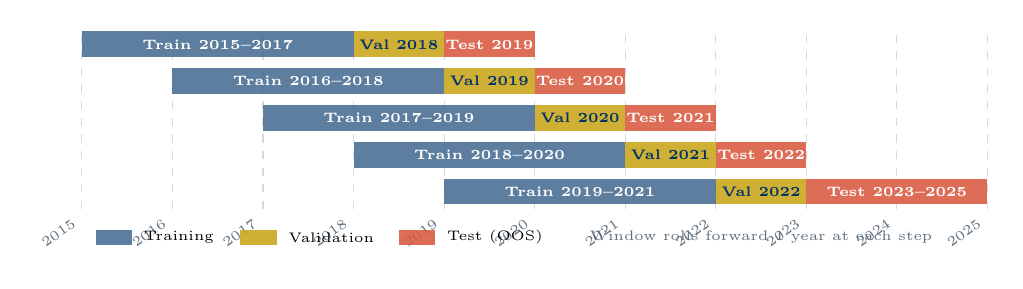
\begin{tikzpicture}[xscale=0.575,yscale=0.82]
			%% Year axis labels
			\foreach \yr/\xp in {2015/0,2016/2,2017/4,2018/6,2019/8,
				2020/10,2021/12,2022/14,2023/16,2024/18,2025/20}{
				\node[font=\tiny,SlateGray,rotate=35,anchor=east] at (\xp,0.08) {\yr};
				\draw[gray!30,dashed] (\xp,0.2) -- (\xp,3.0);
			}
			
			%% Window 1: Train 2015-2017 | Val 2018 | Test 2019
			\fill[Navy!72,opacity=0.88] (0,2.55) rectangle (6,2.95);
			\fill[Gold!90,opacity=0.88] (6,2.55) rectangle (8,2.95);
			\fill[Red!75,opacity=0.88]  (8,2.55) rectangle (10,2.95);
			\node[font=\tiny\bfseries,white] at (3,2.75) {Train 2015--2017};
			\node[font=\tiny\bfseries,Navy]  at (7,2.75) {Val 2018};
			\node[font=\tiny\bfseries,white] at (9,2.75) {Test 2019};
			
			%% Window 2: Train 2016-2018 | Val 2019 | Test 2020
			\fill[Navy!72,opacity=0.88] (2,1.98) rectangle (8,2.38);
			\fill[Gold!90,opacity=0.88] (8,1.98) rectangle (10,2.38);
			\fill[Red!75,opacity=0.88]  (10,1.98) rectangle (12,2.38);
			\node[font=\tiny\bfseries,white] at (5,2.18) {Train 2016--2018};
			\node[font=\tiny\bfseries,Navy]  at (9,2.18) {Val 2019};
			\node[font=\tiny\bfseries,white] at (11,2.18) {Test 2020};
			
			%% Window 3: Train 2017-2019 | Val 2020 | Test 2021
			\fill[Navy!72,opacity=0.88] (4,1.41) rectangle (10,1.81);
			\fill[Gold!90,opacity=0.88] (10,1.41) rectangle (12,1.81);
			\fill[Red!75,opacity=0.88]  (12,1.41) rectangle (14,1.81);
			\node[font=\tiny\bfseries,white] at (7,1.61) {Train 2017--2019};
			\node[font=\tiny\bfseries,Navy]  at (11,1.61) {Val 2020};
			\node[font=\tiny\bfseries,white] at (13,1.61) {Test 2021};
			
			%% Window 4: Train 2018-2020 | Val 2021 | Test 2022
			\fill[Navy!72,opacity=0.88] (6,0.84) rectangle (12,1.24);
			\fill[Gold!90,opacity=0.88] (12,0.84) rectangle (14,1.24);
			\fill[Red!75,opacity=0.88]  (14,0.84) rectangle (16,1.24);
			\node[font=\tiny\bfseries,white] at (9,1.04) {Train 2018--2020};
			\node[font=\tiny\bfseries,Navy]  at (13,1.04) {Val 2021};
			\node[font=\tiny\bfseries,white] at (15,1.04) {Test 2022};
			
			%% Window 5: Train 2019-2021 | Val 2022 | Test 2023-2025
			\fill[Navy!72,opacity=0.88] (8,0.27) rectangle (14,0.67);
			\fill[Gold!90,opacity=0.88] (14,0.27) rectangle (16,0.67);
			\fill[Red!75,opacity=0.88]  (16,0.27) rectangle (20,0.67);
			\node[font=\tiny\bfseries,white] at (11,0.47) {Train 2019--2021};
			\node[font=\tiny\bfseries,Navy]  at (15,0.47) {Val 2022};
			\node[font=\tiny\bfseries,white] at (18,0.47) {Test 2023--2025};
			
			%% Legend
			\fill[Navy!72,opacity=0.88] (0.3,-0.35) rectangle (1.1,-0.12);
			\node[font=\tiny,right] at (1.15,-0.24) {Training};
			\fill[Gold!90,opacity=0.88] (3.5,-0.35) rectangle (4.3,-0.12);
			\node[font=\tiny,right] at (4.35,-0.24) {Validation};
			\fill[Red!75,opacity=0.88]  (7.0,-0.35) rectangle (7.8,-0.12);
			\node[font=\tiny,right] at (7.85,-0.24) {Test (OOS)};
			\node[font=\tiny,SlateGray,right] at (11.0,-0.24)
			{Window rolls forward 1 year at each step};
		\end{tikzpicture}
	\end{frame}
	
	% ===========================================================
	\section{Contributions \& Timeline}
	% ===========================================================
	
	% ── SLIDE 14: EXPECTED CONTRIBUTIONS ───────────────────────
	\begin{frame}{Expected Contributions to Knowledge}
		
		\begin{center}
			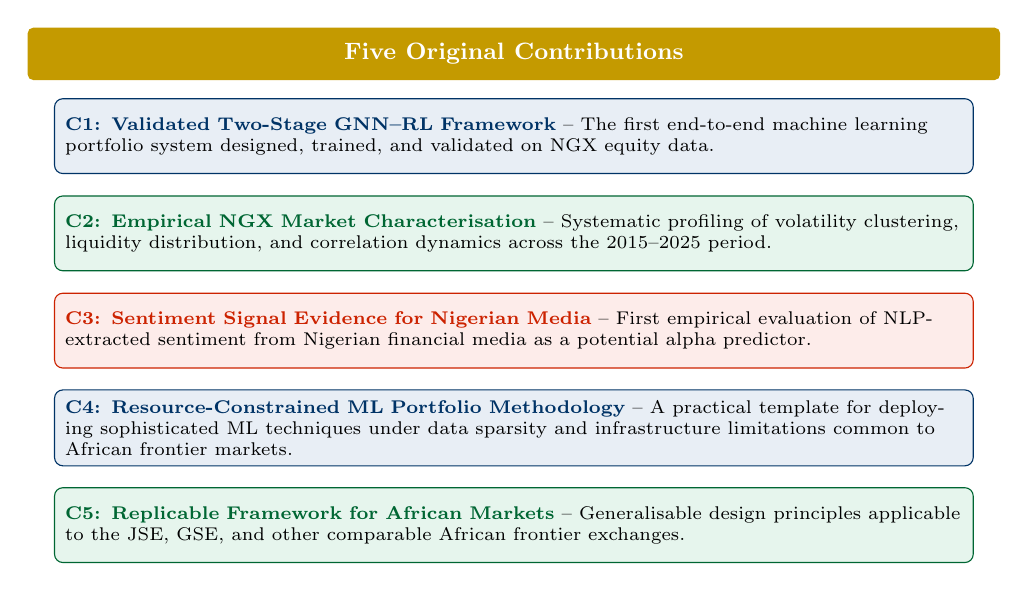
\begin{tikzpicture}[scale=0.95,transform shape]
				
				% Title Bar
				\node[
				rectangle,
				fill=Gold,
				text=white,
				minimum width=13cm,
				minimum height=0.7cm,
				font=\small\bfseries,
				rounded corners=2pt
				] at (0,0)
				{Five Original Contributions};
				
				% Contribution 1
				\node[
				navybox,
				text width=12cm,
				minimum height=1.0cm,
				align=left
%				font=\tiny
				] at (0,-1.1)
				{\textcolor{Navy}{\bfseries C1: Validated Two-Stage GNN--RL Framework} --
					The first end-to-end machine learning portfolio system designed, trained, and validated on NGX equity data.};
				
				% Contribution 2
				\node[
				greenbox,
				text width=12cm,
				minimum height=1.0cm,
				align=left
%				font=\tiny
				] at (0,-2.4)
				{\textcolor{Green}{\bfseries C2: Empirical NGX Market Characterisation} --
					Systematic profiling of volatility clustering, liquidity distribution, and correlation dynamics across the 2015--2025 period.};
				
				% Contribution 3
				\node[
				redbox,
				text width=12cm,
				minimum height=1.0cm,
				align=left
%				font=\tiny
				] at (0,-3.7)
				{\textcolor{Red}{\bfseries C3: Sentiment Signal Evidence for Nigerian Media} --
					First empirical evaluation of NLP-extracted sentiment from Nigerian financial media as a potential alpha predictor.};
				
				% Contribution 4
				\node[
				navybox,
				text width=12cm,
				minimum height=1.0cm,
				align=left
%				font=\tiny
				] at (0,-5.0)
				{\textcolor{Navy}{\bfseries C4: Resource-Constrained ML Portfolio Methodology} --
					A practical template for deploying sophisticated ML techniques under data sparsity and infrastructure limitations common to African frontier markets.};
				
				% Contribution 5
				\node[
				greenbox,
				text width=12cm,
				minimum height=1.0cm,
				align=left
%				font=\tiny
				] at (0,-6.3)
				{\textcolor{Green}{\bfseries C5: Replicable Framework for African Markets} --
					Generalisable design principles applicable to the JSE, GSE, and other comparable African frontier exchanges.};
				
			\end{tikzpicture}
		\end{center}
		
	\end{frame}
	
	% ── SLIDE 15: GANTT CHART (IMPROVED) ───────────────────────
	\begin{frame}{Research Timeline -- 24-Month Plan}
		\vspace{-2pt}
		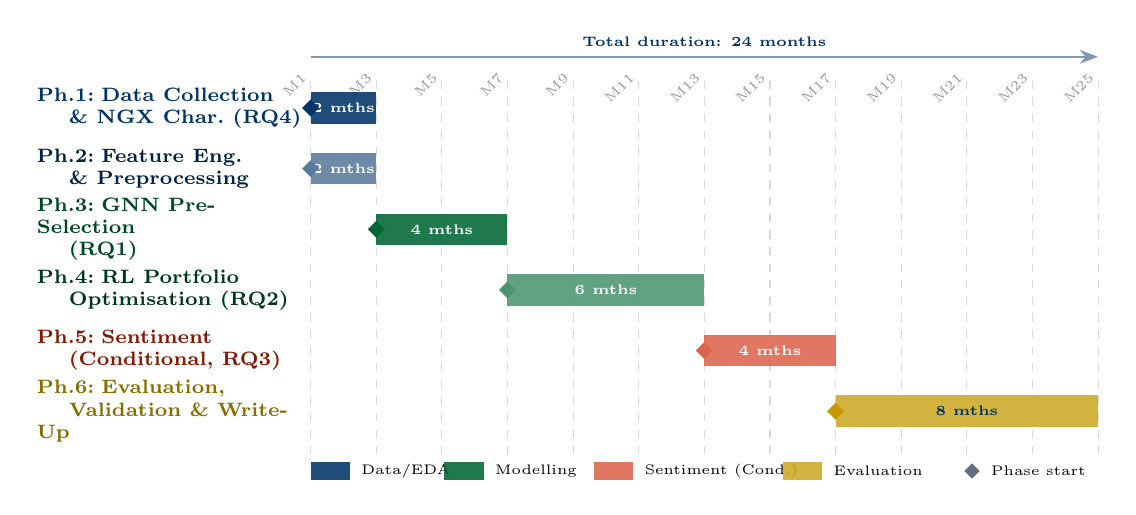
\begin{tikzpicture}
			
			%% ── LABEL COLUMN (left side) ──────────────────────────────
			% Phase labels — right-aligned in a fixed-width column
			\node[font=\scriptsize\bfseries,Navy,right,align=left,
			text width=3.5cm] at (0.0,4.95)
			{Ph.1:\;Data Collection\\\;\quad\& NGX Char.\ (RQ4)};
			\node[font=\scriptsize\bfseries,Navy!65!black,right,align=left,
			text width=3.5cm] at (0.0,4.18)
			{Ph.2:\;Feature Eng.\\\;\quad\& Preprocessing};
			\node[font=\scriptsize\bfseries,Green!70!black,right,align=left,
			text width=3.5cm] at (0.0,3.41)
			{Ph.3:\;GNN Pre-Selection\\\;\quad (RQ1)};
			\node[font=\scriptsize\bfseries,Green!55!black,right,align=left,
			text width=3.5cm] at (0.0,2.64)
			{Ph.4:\;RL Portfolio\\\;\quad Optimisation (RQ2)};
			\node[font=\scriptsize\bfseries,Red!65!black,right,align=left,
			text width=3.5cm] at (0.0,1.87)
			{Ph.5:\;Sentiment\\\;\quad (Conditional, RQ3)};
			\node[font=\scriptsize\bfseries,Gold!70!black,right,align=left,
			text width=3.5cm] at (0.0,1.10)
			{Ph.6:\;Evaluation,\\\;\quad Validation \& Write-Up};
			
			%% ── CHART AREA: starts at x=3.6, spans 10cm for 24 months ─
			%  Each month = 10/24 = 0.4167cm => scale = 0.4167
			
			% Vertical month grid lines and axis labels
			\foreach \m in {0,2,4,...,24}{
				\pgfmathsetmacro{\xg}{3.6 + \m*0.4167}
				\draw[gray!30,dashed] (\xg,0.55) -- (\xg,5.35);
			}
			% Month labels: every even month
			\foreach \m/\lbl in {
				0/M1, 2/M3, 4/M5, 6/M7, 8/M9, 10/M11,
				12/M13, 14/M15, 16/M17, 18/M19, 20/M21, 22/M23, 24/M25}{
				\pgfmathsetmacro{\xg}{3.6 + \m*0.4167}
				\node[font=\tiny,gray!80,rotate=45,anchor=east] at (\xg,5.45) {\lbl};
			}
			
			% Quarter shading bands (subtle)
			\foreach \q in {0,2,...,6}{
				\pgfmathsetmacro{\xs}{3.6 + \q*6*0.4167/6}
			}
			
			%% ── BARS ──────────────────────────────────────────────────
			% Ph.1: months 1-2  (start=0, dur=2)
			\pgfmathsetmacro{\bxs}{3.6}
			\pgfmathsetmacro{\bxe}{3.6 + 2*0.4167}
			\fill[Navy,opacity=0.88] (\bxs,4.75) rectangle (\bxe,5.15);
			\node[font=\tiny\bfseries,white,align=center]
			at ({(\bxs+\bxe)/2},4.95) {2 mths};
			% milestone diamond
			\node[diamond,fill=Navy,minimum size=0.22cm,inner sep=0pt] at (\bxs,4.95) {};
			
			% Ph.2: months 1-2  (parallel with Ph.1, lower row)
			\fill[Navy!65,opacity=0.88] (\bxs,3.98) rectangle (\bxe,4.38);
			\node[font=\tiny\bfseries,white]
			at ({(\bxs+\bxe)/2},4.18) {2 mths};
			\node[diamond,fill=Navy!65,minimum size=0.22cm,inner sep=0pt]
			at (\bxs,4.18) {};
			
			% Ph.3: months 3-6  (start=2, dur=4)
			\pgfmathsetmacro{\bxsa}{3.6 + 2*0.4167}
			\pgfmathsetmacro{\bxea}{3.6 + 6*0.4167}
			\fill[Green,opacity=0.88] (\bxsa,3.21) rectangle (\bxea,3.61);
			\node[font=\tiny\bfseries,white]
			at ({(\bxsa+\bxea)/2},3.41) {4 mths};
			\node[diamond,fill=Green,minimum size=0.22cm,inner sep=0pt]
			at (\bxsa,3.41) {};
			
			% Ph.4: months 7-12  (start=6, dur=6)
			\pgfmathsetmacro{\bxsb}{3.6 + 6*0.4167}
			\pgfmathsetmacro{\bxeb}{3.6 + 12*0.4167}
			\fill[Green!70,opacity=0.88] (\bxsb,2.44) rectangle (\bxeb,2.84);
			\node[font=\tiny\bfseries,white]
			at ({(\bxsb+\bxeb)/2},2.64) {6 mths};
			\node[diamond,fill=Green!70,minimum size=0.22cm,inner sep=0pt]
			at (\bxsb,2.64) {};
			
			% Ph.5: months 13-16  (start=12, dur=4)
			\pgfmathsetmacro{\bxsc}{3.6 + 12*0.4167}
			\pgfmathsetmacro{\bxec}{3.6 + 16*0.4167}
			\fill[Red!70,opacity=0.88] (\bxsc,1.67) rectangle (\bxec,2.07);
			\node[font=\tiny\bfseries,white]
			at ({(\bxsc+\bxec)/2},1.87) {4 mths};
			\node[diamond,fill=Red!70,minimum size=0.22cm,inner sep=0pt]
			at (\bxsc,1.87) {};
			
			% Ph.6: months 17-24  (start=16, dur=8)
			\pgfmathsetmacro{\bxsd}{3.6 + 16*0.4167}
			\pgfmathsetmacro{\bxed}{3.6 + 24*0.4167}
			\fill[Gold!85,opacity=0.88] (\bxsd,0.90) rectangle (\bxed,1.30);
			\node[font=\tiny\bfseries,Navy]
			at ({(\bxsd+\bxed)/2},1.10) {8 mths};
			\node[diamond,fill=Gold,minimum size=0.22cm,inner sep=0pt]
			at (\bxsd,1.10) {};
			
			%% ── LEGEND ────────────────────────────────────────────────
			\fill[Navy,opacity=0.88]    (3.6,0.22) rectangle (4.1,0.45);
			\node[font=\tiny,right] at (4.12,0.34) {Data/EDA};
			\fill[Green,opacity=0.88]   (5.3,0.22) rectangle (5.8,0.45);
			\node[font=\tiny,right] at (5.82,0.34) {Modelling};
			\fill[Red!70,opacity=0.88]  (7.2,0.22) rectangle (7.7,0.45);
			\node[font=\tiny,right] at (7.72,0.34) {Sentiment (Cond.)};
			\fill[Gold!85,opacity=0.88] (9.6,0.22) rectangle (10.1,0.45);
			\node[font=\tiny,right] at (10.12,0.34) {Evaluation};
			\node[diamond,fill=SlateGray,minimum size=0.2cm,inner sep=0pt]
			at (12.0,0.34) {};
			\node[font=\tiny,right] at (12.12,0.34) {Phase start};
			
			%% ── Total duration label ──────────────────────────────────
			\draw[arr,Navy!50] (3.6,5.6) -- (13.6,5.6)
			node[midway,above,font=\tiny\bfseries,Navy]
			{Total duration: 24 months};
		\end{tikzpicture}
	\end{frame}
	
	% ===========================================================
	\section{References}
	% ===========================================================
	
	\begin{frame}[allowframebreaks]{Key References}
		\setbeamertemplate{bibliography item}[text]
		\bibliographystyle{apalike}
		{\tiny\bibliography{references_presentation}}
	\end{frame}
	
	% ── THANK YOU ───────────────────────────────────────────────
	{
		\setbeamertemplate{footline}{}
		\begin{frame}[plain]
			\begin{tikzpicture}[remember picture,overlay]
				\fill[Navy] (current page.south west) rectangle (current page.north east);
				\fill[Gold] (current page.north west) rectangle ++(16cm,-0.2cm);
				\fill[Navy!55] (current page.south west) rectangle ++(16cm,1.4cm);
			\end{tikzpicture}
			\begin{center}
				\vspace{0.5cm}
				\includegraphics[height=1.3cm]{nsuk_logo.jpg}
				\hspace{2cm}
				\includegraphics[height=1.3cm]{ccs_nsuk.jpg}\\[8pt]
				{\color{white}\rule{10cm}{0.4pt}}\\[10pt]
				{\color{Gold}\LARGE\bfseries Thank You}\\[8pt]
				{\color{white}\large Questions \& Discussion}\\[10pt]
				{\color{white}\rule{8cm}{0.3pt}}\\[6pt]
				{\color{white!85}\small\textbf{Isichei, Nnamdi Augustus}
					$\;\mid\;$ kouladoum2022digital}\\[4pt]
				{\color{white!70}\footnotesize Centre for Cyberspace Studies,
					Nasarawa State University, Keffi}\\[5pt]
				{\color{Gold!85}\footnotesize ``Knowledge for Development''}
			\end{center}
		\end{frame}
	}
	
\end{document}